\documentclass[a4paper,11pt,fleqn]{article}%fleqn pour aligner les equations à gauche
\usepackage{../../Styles/Cours}


\newcommand{\chnum}{Chapitre 21}
\newcommand{\chtitle}{Étude de la dynamique d'un système électrique}
\newcommand{\dtype}{Cours}
  
\begin{document}

\maketitle
\section{Courant électrique et intensité}
\begin{minipage}{.6\linewidth}
Un \textbf{courant électrique} correspond à un déplacement de porteurs de charge électrique. Dans les matériaux métalliques, ces porteurs de charge sont es électrons.\\
L'\textbf{intensité du courant} traversant un circuit électrique correspond au \textbf{débit de charges électriques}, c'est à dire à la charge électrique qui traverse une section $S$ du circuit pendant une certaine durée.\\
\end{minipage}
\begin{minipage}{.4\linewidth}
	\centering \begin{tikzpicture}
		\draw[red,line width=1.5] (0,-1) -- (5,-1);
		\draw[-Stealth,red,line width=1.5] (0,-1) to (1,-1); %fil rouge
		\draw (1,-1) node[above,red]{\textbf{I}};
		
		\draw[green!40!blue,line width=2] (3.5,-1) circle(.2);
		\draw[green!40!blue] (3.3,-1) -- (1,-2.25);
		\draw[green!40!blue] (3.7,-1) -- (4.5,-2.25);
		
		\draw (4.5,-3) ellipse(.3 and .75);
		\fill[orange!80] (1,-3.75)rectangle(4.5,-2.25);
		\draw (1,-3.75)rectangle(4.5,-2.25);
		\fill [orange!80] (1,-3) ellipse(.3 and .75);
		\fill [orange!80] (4.5,-3) ellipse(.3 and .75);
		\draw (1,-3) ellipse(.3 and .75);
		\draw[pattern=north east lines] (3,-3) ellipse(.3 and .75);
		\draw (3,-3) ellipse(.3 and .75);
		\draw (3.3,-3) node[right]{S};
		
		\draw[-Stealth,green!40!blue,line width=2] (4.2,-2.7) to (2.5,-2.7);
		\draw[-Stealth,green!40!blue,line width=2] (3.7,-2.5) to (2.2,-2.5);
		\draw[-Stealth,green!40!blue,line width=2] (3.6,-3.2) to (2.1,-3.2);
		\draw[-Stealth,green!40!blue,line width=2] (4,-3.5) to (2.5,-3.5);
		
		\draw (5,-3) node[right,green!40!blue]{Electrons};
	\end{tikzpicture}
\end{minipage}
En régime continu, l'intensité du courant est constante, mais en régime variable, elle peut varier à chaque instant. l'intensité $i(t)$ à un instant donné correspond donc à la charge infinitésimale traversant la section $S$ d'un circuit pendant une durée $dt$ infiniment faible. Mathématiquement, $i(t)$ est donc la dérivée de la charge électrique par rapport au temps :
	$$i(t)=\dfrac{dq}{dt}$$
Remarque : En régime continu, l'intensité du courant est constante. La relation précédente devient donc :
\begin{eqnarray}
	I=\dfrac{Q}{\Delta t} \nonumber & \text{avec : $Q$ la charge totale ayant traversé le circuit}\\
	&\text{$\Delta t$ la durée totale}\nonumber
\end{eqnarray}

Remarque : Les grandeurs électriques sont symbolisées par des lettres majuscules en régime continu ($I$, $U$) et des lettres minuscules en régime variable ($i(t)$, $u(t)$).



\section{Modèle du condensateur}
	\subsection{Définition}
	Un \textbf{condensateur} est un dipôle électrique composé de deux surfaces conductrices (armatures) placées face à face et séparées par un isolant.\\
	Le symbole normalisé d'un condensateur dans un circuit électrique est :
\begin{circuitikz}
	\draw (0,0)
	to[C] (2,0);
\end{circuitikz}

	\subsection{Comportement capacitif}
\begin{minipage}{.6\linewidth}
	Lorsqu'un condensateur est alimenté par un courant électrique continu, des charges électriques opposées s'accumulent sur ses armatures. On dit que ce dipôle a un \textbf{comportement capacitif}. Un tel comportement est également observé dans certaines situations de la vie courante (orages par exemple).\\
\end{minipage}
\begin{minipage}{.4\linewidth}
	\centering \begin{tikzpicture}
		\draw(0,0) -- (2,0);
		\draw(4,0) -- (6,0);
		\draw(2,-1.5) -- (2,1.5);
		\draw(4,-1.5) -- (4,1.5);
		\foreach \k in {-1.5,-1,-.5,0,.5,1,1.5}{
			\draw (2,\k) node[right]{\textbf{+}};
			\draw (4,\k) node[left]{\textbf{-}};
		}
		\draw[-Latex,red,line width=2](0.5,0)to(.6,0);
		\draw[red] (.6,0) node[above] {i};
		\draw (1,0) node[below] {A} node{$\bullet$};
		
		\draw[->,green!90!black,line width=2](1.6,0)to(1.5,0);
		\draw[green!90!black] (1.6,0) node[above] {$e^{-}$};
		
		\draw[->,green!90!black,line width=2](4.6,0)to(4.5,0);
		\draw[green!90!black] (4.6,0) node[above] {$e^{-}$};
		\draw (5,0) node[below] {B} node{$\bullet$};
		
		\draw[-Latex,red,line width=2](5.7,0)to(5.8,0);
		\draw[red] (5.8,0) node[above] {i};
	\end{tikzpicture}
\end{minipage}

L'aptitude d'un condensateur à accumuler des charges électriques est appelée \textbf{capacité}, notée $C$ et exprimée en \textbf{Farad} (\unit{\farad}).\\
Attention à ne pas confondre :\\
\begin{tabular}{|>{\centering}m{9cm}||>{\centering\arraybackslash}m{9cm}|}
	\hline \textbf{C pour capacité} & \textbf{C pour Coulombs}\\
	\hline Grandeur physique correspondant à l'aptitude à accumuler des charges électriques & Unité d'une charge électrique\\
	\hline Exemple : capacité d'un condensateur : $C$ = \num{1} \unit{\farad} & Exemple : charge d'un électron $q_e$ = \num{1,6e-19} \unit{\coulomb}\\
	\hline
\end{tabular}\\

Les condensateurs usuels ont souvent des capacités de \textbf{quelques micro- ou nanofarads} (\unit{\micro\farad} ou \unit{\nano\farad}). De leur coté les superconducteurs, utilisés pour stocker de l'énergie ont des capacités de l'ordre de la centaine de farad.\\
La capacité d'un condensateur dépend de sa \textbf{géométrie} (surface et écartement des armatures) et des \textbf{matériaux} qui le constituent (armature et isolant). Ces variations de capacité sont notamment exploités pour fabriquer des \textbf{capteurs capacitifs} (température, pression, humidité, position, accélération ...).

	\subsection{Relation entre charge, tension et intensité}
\begin{minipage}{.6\linewidth}
	Expérimentalement, on observe que la charge totale $q$ portée par l'armature positive d'un condensateur est proportionnelle à la tension $u_c$ entre ses bornes. Le coefficient de proportionnalité correspond à la capacité $C$ du condensateur.
		\begin{eqnarray}
			q=C \times u_c \nonumber
		\end{eqnarray}
	Il en découle que :
		\begin{eqnarray}
			i(t) = \dfrac{dq}{dt} = C \cdot \dfrac{du_C}{dt} \nonumber 
		\end{eqnarray}
\end{minipage}
\begin{minipage}{.4\linewidth}
	\centering \begin{tikzpicture}
		\draw[-latex,blue!80!white,line width=1.5] (4.75,1.75)to(1.5,1.75);
		\draw[blue!80!white] (3,1.75) node[above] {\large $u_{AB}=u_C$};
		\draw(0,0) -- (2,0);
		\draw(4,0) -- (6,0);
		\draw(2,-1.5) -- (2,1.5);
		\draw(4,-1.5) -- (4,1.5);
		\foreach \k in {-1.5,-1,-.5,0,.5,1,1.5}{
			\draw (2,\k) node[right]{\textbf{+}};
			\draw (4,\k) node[left]{\textbf{-}};
		}
		\draw[-Latex,red,line width=2](0.5,0)to(.6,0);
		\draw[red] (.6,0) node[above] {i};
		\draw (1,0) node[below] {A} node{$\bullet$};
		
		\draw (5,0) node[below] {B} node{$\bullet$};
		\draw[-Latex,red,line width=2](5.7,0)to(5.8,0);
		\draw[red] (5.8,0) node[above] {i};
		
		\draw (2,-1.75) node[below] {\large $q_A$};
		\draw (4.9,-1.75) node[below] {\large $q_B = -q_A$};
	\end{tikzpicture}
\end{minipage}
\newpage
%\begin{landscape}
\begin{minipage}{.7\linewidth}
	\section{Modèle du circuit RC série}
	L'association en série d'un condensateur de capacité $C$ et d'un résistor de résistance $R$ constitue un \textbf{dipôle RC}.
\end{minipage}
\begin{minipage}{.2\linewidth}
	\centering
	\begin{circuitikz}[scale=0.6,transform shape]
		\draw[dashed,red,line width=2] (-1.5,.5)--(1.5,.5)--(1.5,-4)--(-1.5,-4)--cycle;
		\node [above right,red] at (0,.5) {Dipôle RC};
		\draw (0,0) 
		to[R, *-*] (0,-2)
		to[C,l_=$C$, v^<=$u_C$,-*] (0,-3);
		\node [left] at (0,-2) {A};
		\node [left] at (0,-3) {B};	
	\end{circuitikz}
\end{minipage}
	\subsection{Étude de la charge et de la décharge d'un condensateur}
	\begin{tabular}{|m{3cm}|m{7.5cm}|m{7.5cm}|}
		\hline
		 & \centering \textbf{Charge} & \centering \arraybackslash\textbf{Décharge}\\
		\hline \multicolumn{3}{|c|}{\textbf{1. Schéma du circuit électrique}}\\ \hline &\centering \begin{circuitikz}[scale=.8,transform shape]
			\node[cute spdt up, rotate=90] (inter) {};
			\draw   (inter.in)
			to [R,v^<=$u_R$, -*] ++ (0,-2)
			to [C,v^<=$u_C$, -*] ++ (0,-2) coordinate (aux1)
			(inter.out 2)  node[above] {2}
			to [short, -*] ++ (+1,0) |- (aux1)
			(inter.out 1)  node[above] {1}   
			to [short, -*] ++ (-3,0) coordinate (aux2)
			to [vsource,V_<=$E$,i<=$i$, -*]    (aux2 |- aux1)
			to [short, -*] (aux1)
			;
			\node[above left] at (-3.3,.5) {P};
			\node[above] at (0,.5) {K};
			\node[left] at (0,-2.5) {A};
			\node[above left] at (0,-4.5) {B};
			\node[left] at (-3.3,-4.5) {N};
			
			\draw[dashed,red,line width=2] (-2.75,0)--(-.6,0)--(-.6,-4)--(-2.75,-4)--cycle;
			\node [red] at (-1.5,-2) {Maille 1};
			\draw[-latex,red,line width=2](-.6,-1)to(-.6,-.9);
		\end{circuitikz} & \centering\arraybackslash\begin{circuitikz}[scale=.8,transform shape]
		\node[cute spdt down, rotate=90] (inter) {};
		\draw   (inter.in)
		to [R,v_<=$u_R$, -*] ++ (0,-2)
		to [C,v_<=$u_C$, -*] ++ (0,-2) coordinate (aux1)
		(inter.out 2)  node[above] {2}
		to [short, -*] ++ (+3,0) |- (aux1)
		(inter.out 1)  node[above] {1}   
		to [short, -*] ++ (-1,0) coordinate (aux2)
		to [vsource,V_<=$E$,i<=$i$, -*]    (aux2 |- aux1)
		to [short, -*] (aux1)
		;
		\node[above left] at (-1.3,.5) {P};
		\node[above] at (0,.5) {K};
		\node[left] at (0,-2.5) {A};
		\node[above left] at (0,-4.5) {B};
		\node[left] at (-1.3,-4.5) {N};
		
		\draw[dashed,blue,line width=2] (.5,0)--(3,0)--(3,-4)--(.5,-4)--cycle;
		\node [blue] at (1.75,-2) {Maille 2};
		\draw[-latex,blue,line width=2](3,-1)to(3,-.9);
	\end{circuitikz}\\
		\hline \multicolumn{3}{|c|}{\textbf{2. Établissement de l'équation différentielle en $u_C$}:} \\
		\hline Écrire la loi des mailles & D'après la loi des mailles : 
		$$E-u_R-u_C = 0$$
		$$\leftrightarrows u_R + u_C = E$$ & D'après la loi des mailles :
		$$u_R + u_C = 0$$\\
		Utilisation de la loi d'Ohm aux bornes du résistor. & En utilisant la loi d'Ohm, on obtient :
		$$R\times i + u_C = E $$ & En utilisant la loi d'Ohm, on obtient :
		$$R\times i + u_C = 0$$\\
		Utiliser la relation entre charge et intensité. & Sachant que $i=\dfrac{dq}{dt}$, on a :
		$$R\times \dfrac{dq}{dt}+u_C=E$$ & Sachant que $i=\dfrac{dq}{dt}$, on a :
		$$R\times \dfrac{dq}{dt}+u_C=0 $$\\
		Utiliser la relation entre charge et tension. & Comme $q=C\cdot u_C$, alors :
		$$R\times C\dfrac{du_C}{dt}+u_C=E $$
		On obtient ainsi l'équation différentielle en $u_C$& Comme $q=C\cdot u_C$, alors :
		$$R\times C\dfrac{du_C}{dt}+u_C=0$$
	On obtient ainsi l'équation différentielle en $u_C$\\
 \hline
 \end{tabular}\\
% \newpage

 \begin{tabular}{|m{3cm}|m{7.5cm}|m{7.5cm}|}
    \hline \multicolumn{3}{|c|}{\textbf{3. Résolution de l'équation différentielle}}\\
	\hline Écrire l'équation sous la forme $y'+ay=b$& L'expression précédente devient :
	\begin{eqnarray}
		\dfrac{du_C}{dt} + \dfrac{1}{RC} \times u_C = \dfrac{E}{RC} \nonumber
	\end{eqnarray} & L'expression précédente devient :
		\begin{eqnarray}
			\dfrac{du_C}{dt} + \dfrac{1}{RC} \times u_C = 0 \nonumber
		\end{eqnarray}\\
	Donner l'expression générale des solutions à cette équation. & Les solutions à cette équation sont de la forme : 
	\begin{eqnarray}
		u_C(t)=K_1\times e^{-\dfrac{t}{RC}}+E \nonumber
	\end{eqnarray} & Les solutions à cette équation sont de la forme : 
	\begin{eqnarray}
		u_C(t)=K_2\times e^{-\dfrac{t}{RC}} \nonumber
	\end{eqnarray}\\
	Déterminer la solution particulière à l'aide des conditions initiales. & On détermine $K$ à l'aide des conditions initiales : A t = 0 s, le condensateur est déchargé,
	\begin{eqnarray}
		u_C(0)=0\nonumber\\
		\leftrightarrow K_1 \times e^{-\dfrac{0}{RC}}+E=0 \nonumber\\
		\leftrightarrow K_1 \times 1 + E =0\nonumber \\
		\leftrightarrow K_1 =-E\nonumber
	\end{eqnarray}
	Ainsi : 
	\begin{eqnarray}
		u_C(t)=-E\times e^{-\dfrac{t}{RC}}+E\nonumber\\
		\leftrightarrow u_C(t)=E\left(1-e^{-\dfrac{t}{RC}}\right)\nonumber
	\end{eqnarray} & On détermine $K$ à l'aide des conditions initiales : A t = 0 s, le condensateur est chargé,
	\begin{eqnarray}
		u_C(0)=E\nonumber\\
		\leftrightarrow K_2 \times e^{-\dfrac{0}{RC}}=E \nonumber\\
		\leftrightarrow K_2 \times 1 =E\nonumber \\
		\leftrightarrow K_2 =E\nonumber
	\end{eqnarray}
	Ainsi : 
	\begin{eqnarray}
		u_C(t)=E\times e^{-\dfrac{t}{RC}}\nonumber
\end{eqnarray}\\
	\hline \textbf{4. Allure de la courbe} & 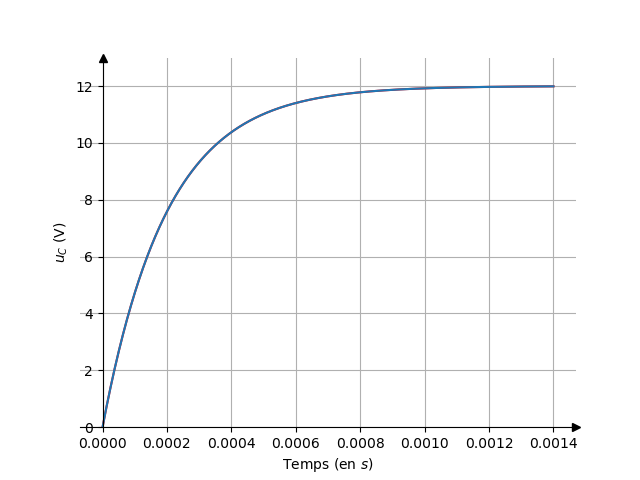
\includegraphics[scale=.4]{Ressources/TSPE_C11_Cours_Fig1.png}&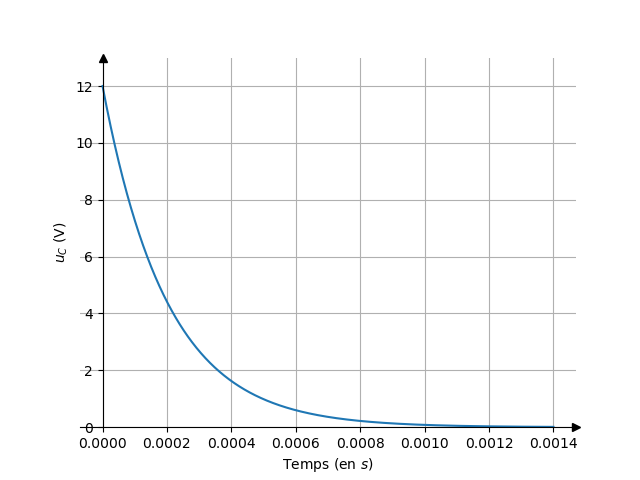
\includegraphics[scale=.4]{Ressources/TSPE_C11_Cours_Fig2.png}\\
	\hline
	\end{tabular}
%\end{landscape}

	\subsection{Temps caractéristique}
	L'expression de $u_C(t)$ fait intervenir le produit $R\times C$. Ce produit est homogène à un temps. Il est appelé \textbf{temps caractéristique} ou \textbf{constante de temps} du circuit RC série. il est noté $\tau$ (tau) et s'exprime en secondes.
	\begin{eqnarray}
		\tau = R\times C\nonumber
	\end{eqnarray}
	Les solutions $u_C(t)$ des équations différentielles peuvent donc s'exprimer en fonction de $\tau$ :\\
	\begin{table}[h!]
		\centering \begin{tabular}{|>{\centering}m{5cm}|>{\centering\arraybackslash}m{5cm}|}
		\hline \textbf{\textsc{Charge}} & \textbf{\textsc{Décharge}}\\
		\hline $u_C(t)=E\left(1-e^{-\dfrac{t}{\tau}}\right)$ & $u_C(t)=E\times e^{-\dfrac{t}{\tau}}$\\
		\hline
		\end{tabular}
	\end{table}

\noindent
	\begin{minipage}{.5\linewidth}
		$\tau$ peut être déterminé graphiquement de plusieurs manières : 
		\begin{itemize}
			\item en traçant la \textbf{tangente à l'origine} et l'\textbf{asymptote} horizontale à la courbe $u_C(t)$; $\tau$ est alors l'abscisse su point d'intersection
			\item en représentant le point pour lequel la tension \textbf{$u_C$ atteint 63 \% de E}; $\tau$ est alors l'abscisse de ce point.
		\end{itemize}
	\end{minipage}
	\begin{minipage}{.4\linewidth}
		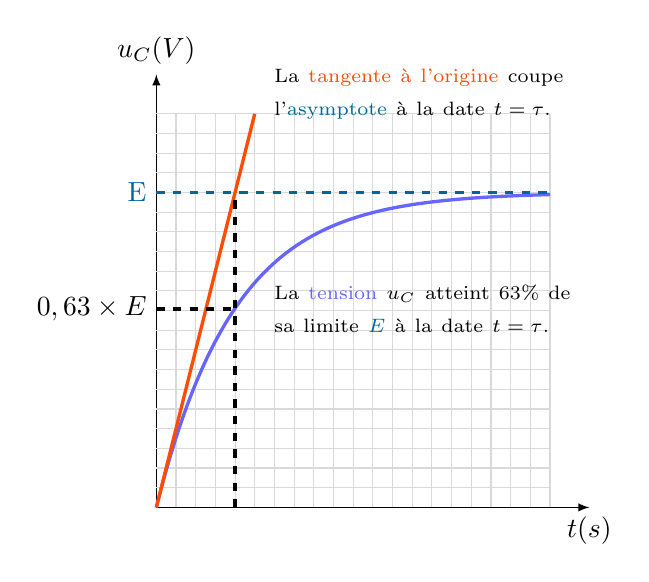
\begin{tikzpicture}[scale=.5]
			\draw[-latex] (0,0) to (0,11);
			\draw[-latex] (0,0) to (11,0);
			\foreach \k in {.5,1,...,10}{
				\draw[gray!30] (0,\k) to (10,\k);
				\draw[gray!30] (\k,0) to (\k,10); }
			\draw [domain=0:10,samples = 600,blue!60,line width = 1.2pt] plot (\x,{8*(1-exp(-\x/2))});%courbe
			\draw[dashed,green!40!blue,line width=1.2pt] (0,8) -- (10,8);%asymptote
			\draw [domain=0:2.5,samples = 600,orange!60!red,line width = 1.2pt] plot (\x,{(8/2)*\x});%tangente
			\draw[dashed,line width=1.2pt] (2,0)--(2,8);
			\draw[dashed,line width=1.2pt] (0,5.04)--(2,5.04);
			
			\node[above] at (0,11)  {$u_C (V)$};
			\node[below] at (11,0)  {$t (s)$};
			\node[left,green!40!blue] at (0,8)  {E};
			\node[left] at (0,5.04)  {$0,63 \times E$};
			%\node[left] at (3,5.04)  {La tension $u_C$ atteint 63 \% de sa limite $E$ à la date $t=\tau$.};
			\node at (7,5.04) [text width=4cm]{\scriptsize La \textcolor{blue!60}{tension} $u_C$ atteint 63\% de sa limite \textcolor{green!40!blue}{$E$} à la date $t=\tau$.};
			\node at (7,10.5) [text width=4cm]{\scriptsize La \textcolor{orange!60!red}{tangente à l'origine} coupe l'\textcolor{green!40!blue}{asymptote} à la date $t=\tau$.};
		\end{tikzpicture}
	\end{minipage}

\noindent
	\begin{minipage}{.6\linewidth}
		$\tau$ permet de déterminer la durée de la charge ou de la décharge d'un dipôle RC. Plus $\tau$ est grand, plus la durée de charge ou de décharge est grande. Au bout de $5\tau$, on considère que le condensateur est chargé ou déchargé (la tension $u_C$ a atteint sa valeur finale à 1 \% près). Le \textbf{régime transitoire} est alors considéré comme terminé et un \textbf{régime permanent stationnaire} s'établir.
	\end{minipage}
\begin{minipage}{.4\linewidth}
	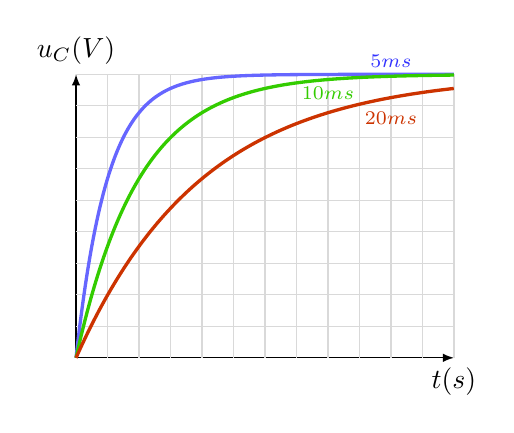
\begin{tikzpicture}[scale=.8]
		\draw[-latex] (0,0) to (0,4.5);
		\draw[-latex] (0,0) to (6,0);
		\foreach \k in {.5,1,...,4.5}{
			\draw[gray!30] (0,\k) to (6,\k);}
		\foreach \k in {.5,1,...,6}{
			\draw[gray!30] (\k,0) to (\k,4.5); }
		\draw [domain=0:6,samples = 1000,blue!60,line width = 1.2pt] plot (\x,{4.5*(1-exp(-\x/.5))});%courbe 5ms
		\node at (5,4.7) {\scriptsize \textcolor{blue!80}{$5ms$}};
		
		\draw [domain=0:6,samples = 1000,green!80!red,line width = 1.2pt] plot (\x,{4.5*(1-exp(-\x))});%courbe 10ms
		\node at (4,4.2) {\scriptsize \textcolor{green!80!red}{$10ms$}};
		
		\draw [domain=0:6,samples = 1000,red!80!green,line width = 1.2pt] plot (\x,{4.5*(1-exp(-\x/2))});%courbe 20ms
		\node at (5,3.8) {\scriptsize \textcolor{red!80!green}{$20ms$}};
		
		\node[above] at (0,4.5)  {$u_C (V)$};
		\node[below] at (6,0)  {$t (s)$};
	\end{tikzpicture}
\end{minipage}

\noindent
\begin{minipage}{.5\linewidth}
	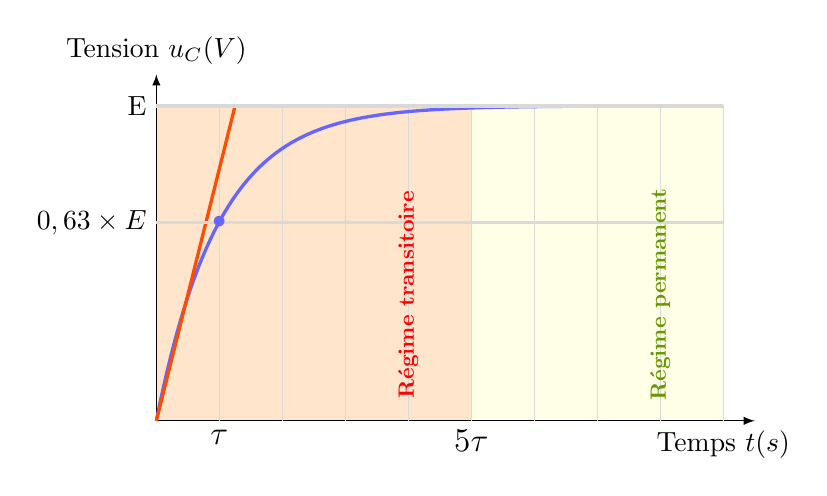
\begin{tikzpicture}[scale=.4]
		\fill[orange!20] (0,0)--(0,10)--(10,10)--(10,0)--cycle;
		\fill[yellow!10] (10,0)--(10,10)--(18,10)--(18,0)--cycle;
		
		\draw[-latex] (0,0) to (0,11);
		\draw[-latex] (0,0) to (19,0);
		\foreach \k in {2,4,...,18}{
			\draw[gray!30] (\k,0) to (\k,10); }
		\draw [domain=0:18,samples = 600,blue!60,line width = 1.2pt] plot (\x,{10*(1-exp(-\x/2))});%courbe
		
		\draw [domain=0:2.5,samples = 600,orange!60!red,line width = 1.2pt] plot (\x,{(8/2)*\x});%tangente

		\draw[gray!30,line width=1.2pt] (0,6.3)--(18,6.3);
		\draw[gray!30,line width=1.2pt] (0,10)--(18,10);
		
		\node[above] at (0,11)  {Tension $u_C (V)$};
		\node[below] at (18,0)  {Temps $t (s)$};
		\node[left] at (0,10)  {E};
		\node[left] at (0,6.3)  {$0,63 \times E$};
		\draw[blue!60] (2,6.3) node{$\bullet$};
		
		\node[below] at (2,0)  {\large $\tau$};
		\node[below] at (10,0)  {\large $5\tau$};
		
		\node[red,rotate = 90,scale=.8] at (8,4) {\textbf{Régime transitoire}};
		\node[green!60!red,rotate = 90,scale=.8] at (16,4) {\textbf{Régime permanent}};
		
		
	\end{tikzpicture}
\end{minipage}
\begin{minipage}{.5\linewidth}
	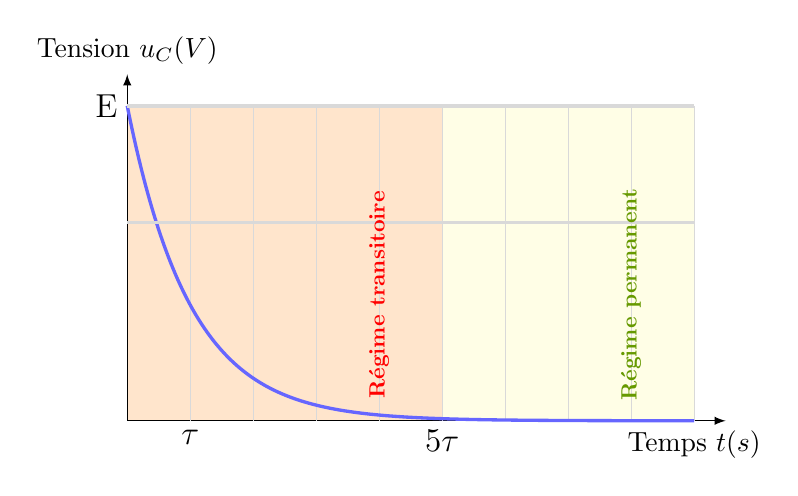
\begin{tikzpicture}[scale=.4]
		\fill[orange!20] (0,0)--(0,10)--(10,10)--(10,0)--cycle;
		\fill[yellow!10] (10,0)--(10,10)--(18,10)--(18,0)--cycle;
		
		\draw[-latex] (0,0) to (0,11);
		\draw[-latex] (0,0) to (19,0);
		\foreach \k in {2,4,...,18}{
			\draw[gray!30] (\k,0) to (\k,10); }
		\draw [domain=0:18,samples = 600,blue!60,line width = 1.2pt] plot (\x,{10*exp(-\x/2)});%courbe
		
		%\draw [domain=0:2.5,samples = 600,orange!60!red,line width = 1.2pt] plot (\x,{(8/2)*\x});%tangente
		
		\draw[gray!30,line width=1.2pt] (0,6.3)--(18,6.3);
		\draw[gray!30,line width=1.2pt] (0,10)--(18,10);
		
		\node[above] at (0,11)  {Tension $u_C (V)$};
		\node[below] at (18,0)  {Temps $t (s)$};
		\node[left] at (0,10)  {\large E};
		%\node[left] at (0,6.3)  {\large $0,63 \times E$};
		%\draw[blue!60] (2,6.3) node{$\bullet$};
		
		\node[below] at (2,0)  {\large $\tau$};
		\node[below] at (10,0)  {\large $5\tau$};
		
		\node[red,rotate = 90,scale=.8] at (8,4) {\textbf{Régime transitoire}};
		\node[green!60!red,rotate = 90,scale=.8] at (16,4) {\textbf{Régime permanent}};
		
		
	\end{tikzpicture}
\end{minipage}
\end{document}
\end{document}
